\documentclass{beamer}
\usepackage{listings}
\beamertemplatenavigationsymbolsempty
\hypersetup{pdfstartview={Fit}}%Pdf fit page as default
\usecolortheme{beetle}

\title{String processing}
\author{Robin Jadoul}
\date{30 januari 2016}

\institute
{
    
\includegraphics[height=65px]{img/Icon.png}
}

\AtBeginSection[]
{
  \begin{frame}
    \frametitle{Table of Contents}
    \tableofcontents[currentsection]
  \end{frame}
}

\AtBeginSubsection[]
{
  \begin{frame}
    \frametitle{Table of Contents}
    \tableofcontents[currentsection,currentsubsection]
  \end{frame}
}

\begin{document}
\frame{\titlepage}

\section[Ad hoc]{Ad hoc}
\frame{
    \frametitle{Ad hoc}
    \begin{itemize}[<+->]
        \item Straightforward solution
        \item See CP3, section 6.3 (pages 236 - 240)

        \item If you know regular expressions, C++ 11 has those as well
    \end{itemize}
}


\section[Tries]{Tries}
\frame
{
    \frametitle{Trie}
    \framesubtitle{Properties}
    \begin{itemize}[<+->]
        \item \textless Re\emph{trie}val (but can be pronounce as either \emph{tree} or \emph{try})
        \item Store a set of words (with or without associated values)
        \item insert/retrieve in $ O(S) $, with S the length of the string
        \item Allows for non-exact matches (\textless\textgreater ~ set/map)
    \end{itemize}
}

\frame
{
    \frametitle{Trie}
    \framesubtitle{Structure}

    \begin{itemize}[<+->]
        \item Tree structure
        \item Stores the \emph{path} for the string instead of the string
        \item Edges labeled with single characters
        \item If the last character of a stored word, marked (+ associated value)
        \item Can vary in type of \emph{character} (bits/ints/\dots)
        \item Can be compressed by eliminating successive single-edge nodes
    \end{itemize}
}

\frame
{
    \frametitle{Trie}
    \framesubtitle{Structure}

    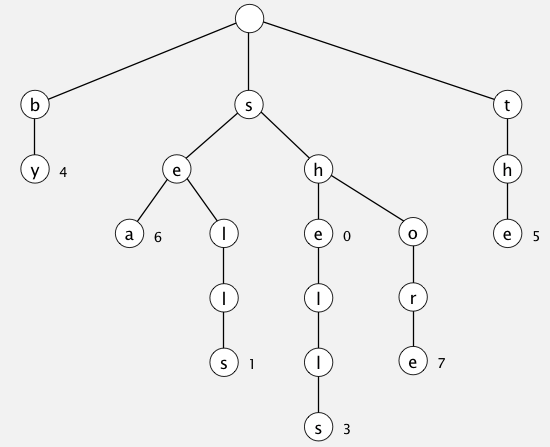
\includegraphics[width=0.8\textwidth]{img/trie.png}
}

\frame
{
    \frametitle{Trie}
    \framesubtitle{Usage}
    \begin{itemize}[<+->]
        \item Spelling suggestions
        \item Autocompletion
        \item Bioinformatics (DNA/RNA)
        \item Alphabetical ordering / sorting
        \item (Similar to structure for Aho-Corasick)
        \item (Basis for \emph{suffix tree})
    \end{itemize}
} 

\begin{frame}[fragile]
    \frametitle{Trie}
    \framesubtitle{Code}
    \lstinputlisting[language=C++,basicstyle=\tiny,keywordstyle=\color{blue},firstline=1,lastline=9]{src/trie.cpp}
\end{frame}

\begin{frame}[fragile]
    \frametitle{Trie}
    \framesubtitle{Code}
    \lstinputlisting[language=C++,basicstyle=\tiny,keywordstyle=\color{blue},firstline=11,lastline=22]{src/trie.cpp}
\end{frame}

\begin{frame}[fragile]
    \frametitle{Trie}
    \framesubtitle{Code}
    \lstinputlisting[language=C++,basicstyle=\tiny,keywordstyle=\color{blue},firstline=24,lastline=33]{src/trie.cpp}
\end{frame}


\section[String matching]{String matching}
\subsection[Naive]{Naive}
\frame{
    \frametitle{Naive matching}
    \framesubtitle{principle}
    
    \begin{itemize}[<+->]
        \item Straightforward
        \item Check for match at each index
        \item Usually, use the one in the standard library, don't write your own
        \item $ O(s * p) $ (s = length of string, p = length of pattern)
    \end{itemize}
}

\begin{frame}[fragile]
    \frametitle{Naive matching}
    \framesubtitle{Code}

    \lstinputlisting[language=C++,basicstyle=\tiny,keywordstyle=\color{blue}]{src/naive-matching.cpp}
\end{frame}

\subsection[Rabin-Karp]{Rabin-Karp}
\frame{
    \frametitle{Rabin-Karp}
    \framesubtitle{Idea}

    \begin{itemize}[<+->]
        \item Checking for a match with the pattern: $O(n)$
        \item Faster possible?
        \item What about hashes, integer comparison = $O(n)$
        \item We still need a $O(1)$ way to generate the hashes.
        \item Useful for multiple same-length patterns (check all hashes)
    \end{itemize}
}

\frame{
    \frametitle{Rabin-Karp}
    \framesubtitle{Polynomial hashing}

    \begin{itemize}[<+->]
        \item Generate successive hashes of the same length as the pattern (and hash the pattern)
        \item Polynomial hashing: the string is an integer in some base $B$ (usually prime)
        \item $s_i,s_{i+1},\ldots,s_{i+k-1} = s_i \times B^{k-1} + s_{i+1} \times B^{k-2} + \ldots + s_{i+k-1} \times B^{0}$
        \item Too big $\Rightarrow$ modulo $H$ (usually prime)
        \item Watch out for false positives
    \end{itemize}
}

\frame{
    \frametitle{Rabin-Karp}
    \framesubtitle{Rolling hashes}

    \begin{itemize}[<+->]
        \item Once we have a hash, it's easy to compute the next
        \item $s_{i+1},s_{i+2},\ldots,s_{i+k} = ((s_i,\ldots,s_{i+k-1}) - s_i \times B^{k-1}) \times B) + s_{i+k}$
        \item A rolling hash \emph{frame}
        \item $O(1)$
    \end{itemize}
}

\frame{
    \frametitle{Rabin-Karp}
    \framesubtitle{Collision strategies}

    \begin{itemize}[<+->]
        \item If equal hashes $\Rightarrow$ compare the strings explicitely
        \item Worst case, still $O(n^2)$
        \item \emph{Gambling}: keep 2 hashes (with distinct $B$ and $H$)
        \item Collision chance is low, if the two hashes match, guess it's correct
        \item $\Rightarrow$ triple hashing, \dots
    \end{itemize}
}

\frame{
    \frametitle{Rabin-Karp}
    \framesubtitle{code}

    \lstinputlisting[language=C++,basicstyle=\tiny,keywordstyle=\color{blue},firstline=4,lastline=15]{src/rabin-karp.cpp}
}

\frame{
    \frametitle{Rabin-Karp}
    \framesubtitle{code}

    \lstinputlisting[language=C++,basicstyle=\tiny,keywordstyle=\color{blue},firstline=17,lastline=34]{src/rabin-karp.cpp}
}

\frame{
    \frametitle{Rabin-Karp}
    \framesubtitle{code}

    \lstinputlisting[language=C++,basicstyle=\tiny,keywordstyle=\color{blue},firstline=36,lastline=53]{src/rabin-karp.cpp}
}

\subsection[Z-algorithm]{Z-algorithm}
\frame{
    \frametitle{Z-algorithm}
    \framesubtitle{terminology}
    
    \begin{itemize}[<+->]
        \item Z-box = substring that matches with a prefix from the string
        \item Z-score $Z_i(S)$ = length of Z-box starting at index $i$
    \end{itemize}

    \begin{center}
        \only<3->{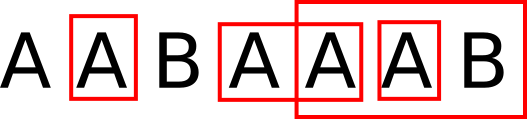
\includegraphics{img/z-box.png}}
    \end{center}

    \pause

    \begin{center}
    \only<4->{
    \begin{tabular}{|l|c|c|c|c|c|c|c|}
        \hline
        letter&A&A&B&A&A&A&B\\
        \hline
        Z-score&7&1&0&2&3&1&0\\
        \hline
    \end{tabular}}
    \end{center}
}

\frame{
    \frametitle{Z-algorithm}
    \framesubtitle{Matching}

    \begin{itemize}[<+->]
        \item $P$ = pattern
        \item $S$ = search string
        \item $\$$ = sentinel (not part of alphabet)
        \item return $i$ for each $i > 0$ where $Z_i(P\$S) = |P|$
    \end{itemize}
}

\frame{
    \frametitle{Z-algorithm}
    \framesubtitle{Calculating Z-scores}

    \begin{itemize}[<+->]
        \item Naive $\Rightarrow$ $O(n^2)$, possible in $O(n)$
        \item Keep track of the Z-box with right end furthest to the right (bounds: $[l, r]$)
        \item if current character in $[l, r]$: look at corresponding character in prefix (computed previously)
        \item expand if grows beyond $r$, update $[l, r]$
        \item else: calculate explicitely, update $[l, r]$
        \item (Nicely illustrated: https://www.cs.umd.edu/class/fall2011/cmsc858s/Lec02-zalg.pdf)
    \end{itemize}
}

\begin{frame}[fragile]
    \frametitle{Z-algorithm}
    \framesubtitle{code}

    \lstinputlisting[language=C++,basicstyle=\tiny,keywordstyle=\color{blue},firstline=4,lastline=28]{src/z-algo.cpp}
\end{frame}

\begin{frame}[fragile]
   \frametitle{Z-algorithm}
   \framesubtitle{code}

   \lstinputlisting[language=C++,basicstyle=\tiny,keywordstyle=\color{blue},firstline=29,lastline=44]{src/z-algo.cpp}
\end{frame}

\subsection[Knuth-Morris-Pratt]{Knuth-Morris-Pratt}
\frame{
    \frametitle{Knuth-Morris-Pratt}
    \framesubtitle{Idea}

    \begin{itemize}[<+->]
        \item Don't restart a match every time
        \item Fail smart
        \item Re-use previous (partial) match information
        \item Precompute possible \emph{sub}matches
    \end{itemize}
}

\frame{
    \frametitle{Knuth-Morris-Pratt}
    \framesubtitle{Idea}

    \begin{itemize}[<+->]
        \item How to choose the next possible match?
        \item Next possible partially matched pattern = longest proper suffix (of the partial match) that is a prefix
        \item (What is this in terms of Z-boxes?)
        \item Precompute and keep the length of this suffix/prefix in an array (call this $L$)
        \item $L[i]$ = length of that prefix for $S[0..i-1]$ (inclusive)
    \end{itemize}
}

\frame{
    \frametitle{Knuth-Morris-Pratt}
    \framesubtitle{Precomputation}

    \begin{itemize}[<+->]
        \item $L[0] = -1$ (could be $0$, but this eliminates a few checks)
        \item $L[1] = 0$ (it should be a \emph{proper} suffix)
        \item Search for the next \emph{parent} in $L$ that can be expanded with the current character
        \item $L[i] = j + 1$ ($j$ is the length of the \emph{parent}'s match)
        \item If none can be found: $L[i] = 0$
    \end{itemize}
}

\frame{
    \frametitle{Knuth-Morris-Pratt}
    \framesubtitle{Matching}

    \begin{itemize}[<+->]
        \item Precompute the suffix lengths ($L$) of the pattern
        \item Re-use partial matches using $L$ while matching
        \item Very similar to the actual precomputation
        \item $O(S + P)$
    \end{itemize}
}

\frame{
    \frametitle{Knuth-Morris-Pratt}
    \framesubtitle{code}

    \lstinputlisting[language=C++,basicstyle=\tiny,keywordstyle=\color{blue},firstline=4,lastline=16]{src/kmp.cpp}
}

\frame{
    \frametitle{Knuth-Morris-Pratt}
    \framesubtitle{code}

    \lstinputlisting[language=C++,basicstyle=\tiny,keywordstyle=\color{blue},firstline=18,lastline=32]{src/kmp.cpp}
}


\section[Exercises]{Exercises}
 
\subsection{Exercises}
\begin{itemize}
 \item \url{http://codeforces.com/contest/406/problem/D}
\end{itemize}

\end{document}
